\newcommand{\byr}{Br}

\section{Требования к пояснительной записке}

\subsection{Общие положения}

\subsubsection{} 
Пояснительную  записку  выполняют  рукописным  способом  или  с применением печатающих и графических устройств вывода ЭВМ. 

При рукописном способе используют шариковую ручку с пастой черного или синего, или фиолетового цвета. Высота букв и цифр должна быть не менее 3,5 мм. 

При применении текстовых редакторов ЭВМ печать производится шрифтом 13\,--\,14  пунктов  с  межстрочным  интервалом,  позволяющим  разместить  
40\,\( \pm \)\,3 строки на странице. 

Номера  разделов,  подразделов,  пунктов и подпунктов следует выделять полужирным  шрифтом.  Заголовки  разделов  допускается  оформлять  полужирным шрифтом размером 14\,--\,16 пунктов, а заголовки подразделов полужирным шрифтом размером 14 пунктов. 

Для  акцентирования  внимания  на  определенных  терминах  допускается применять шрифты разной гарнитуры. 

\subsubsection{}
Текст располагают на одной стороне листа формата А4 с соблюдением размеров полей и интервалов, указанных в приложении Л.

\subsubsection{}
Абзацы в тексте начинают отступом, равным 15\,--\,17 мм при выполнении  записи  рукописным  способом  или  пяти  знакам  при  применении  печатающего устройства вывода ЭВМ.

\subsubsection{} 
Все  части  пояснительной  записки  необходимо  излагать  только  на одном языке "--- на русском или белорусском, или на одном из иностранных языков, например английском или немецком.

\subsubsection{} 
Описки и графические неточности, обнаруженные в тексте пояснительной записки, выполненной рукописным способом, допускается исправлять подчисткой, закрашиванием белой краской и нанесением на том же месте исправленного текста. Помарки и следы не полностью удаленного прежнего текста не допускаются.

\subsubsection{} 
Пояснительная записка\footnote{Пример сноски} должна быть оформлена в жестком переплете (в специальной папке для дипломных проектов или работ).


\subsection{Рубрикации, заголовки и содержание}

\subsubsection{} 
Текст пояснительной записки разделяют на логически сопряженные части "--- разделы, а при необходимости и подразделы. Как разделы, так и подразделы могут состоять из одного или нескольких пунктов.

\subsubsection{}
Разделы должны быть пронумерованы арабскими цифрами без точки  в конце  и записанные с абзацного отступа. Подразделы 
нумеруют в пределах раздела, к которому они относятся.

\subsubsection{}
Иногда внутри подраздела необходимо выделить более мелкие смысловые подразделения – пункты, например: характеристики устройств и функциональных элементов технической системы; обоснование этапов планируемого эксперимента, характеристики аппаратов и приборов, необходимых для испытаний; показатели качества технической системы в различных режимах ее работы и т.\,д. В подобных случаях пункты нумеруют в пределах подраздела. Цифровой индекс пункта должен состоять из номеров раздела, подраздела и пункта, разделенных точками, и записан с абзацного отступа. 

Пункты при необходимости могут быть разбиты на подпункты, которые нумеруются в пределах каждого пункта. 

\subsubsection{}
Если в пояснительной записке выделены только разделы, то пункты нумеруют в пределах раздела.

\subsubsection{}
Каждый раздел и подраздел должен иметь краткий и ясный заголо-вок. Пункты, как правило, заголовков не имеют. Заголовки разделов записывают прописными буквами без точки в конце заголовка. Заголовки подразделов записывают стро чными буквами, начиная с первой прописной. Заголовки не подчеркивают. Перен осы слов в заголовках не допускаются. Если заголовок состоит из двух предложений, их разделяют точкой.

В случае, когда заголовки раздела или подраздела занимают несколько строк, то строки выравниваются  по первой букве  заголовка  в соответствии с приложением Л\footnote{Его тут нет}.

\subsubsection{}
Каждый раздел пояснительной записки рекомендуется начинать с новой страницы. 

Между заголовком раздела (подраздела) и текстом оставляют пробельную строку "--- при компьютерном способе выполнения  записки;  интервал  шириной 15\,мм "--- при рукописном способе (см.~приложение Л).

Между заголовками разделов и входящих в него подразделов допускается помещать небольшой вводный текст, предваряющий подраздел.

\subsubsection{}
Перечень всех разделов и подразделов, включающий порядковые номера и заголовки, оформляют в виде содержания "--- обязательного элемента пояснительной записки. Содержание помещают непосредственно за заданием на проектирование и включают в общую нумерацию страниц.

Слово \MakeUppercase{содержание} записывают прописными буквами полужирным шрифтом 14 "--- 16 пунктов и располагают по центру строки. Между словом \MakeUppercase{содержание} и самим содержанием оставляют промежуток, равный пробельной строке. В содержании заголовки выравнивают, соподчиняя по разделам, подразделам и пунктам (если последние имеют заголовки), смещая вертикали вправо относительно друг друга на 2 знака.

% Пример организации пустых разделов
\section*{Введение}
\label{sec:intro}
\addcontentsline{toc}{section}{Введение}
Разделы начинаются с новой страницы автоматически. Подразделы и подподразделы "--- нет.


\section{Анализ нескорректированной системы управления}
\label{sec:analysys_equations}
Пример того, как оформить рисунок, смотри на рисунке~\ref{fig:fire_alarms}
\begin{figure}[ht]
\centering
  \begin{subfigure}[b]{0.45\textwidth} 
    \centering
    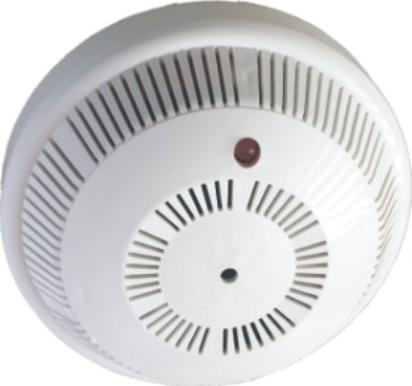
\includegraphics[scale=0.85]{avt_pozh_izv.jpg}  
    \caption{}
  \end{subfigure}
  \begin{subfigure}[b]{0.45\textwidth} 
    \centering
    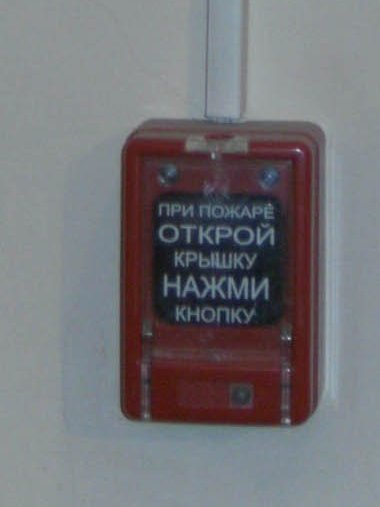
\includegraphics[scale=1.2]{ruch_pozh_izv.jpg}  
    \caption{}
  \end{subfigure}
  \caption{ а  "--- автономный пожарный извещатель;
            б  "--- ручной пожарный извещатель.}
  \label{fig:fire_alarms}
\end{figure}


\subsection{Анализ исходных данных} 
\label{sec:analysys_data}
Смотри как выглядит таблица~\ref{table:econ:function_sizes}, она является примером оформления таблиц. Ее расположение выбирается подпибается автоматичеки для лучшей заполняемости страниц.
\begin{table}[ht]
\caption{Перечень и объем функций программного модуля}
\label{table:econ:function_sizes}
\centering
  \begin{tabular}{| >{\centering}m{0.12\textwidth} 
                  | >{\raggedright}m{0.40\textwidth} 
                  | >{\centering}m{0.18\textwidth} 
                  | >{\centering\arraybackslash}m{0.18\textwidth}|}

  \hline
         \multirow{2}{0.12\textwidth}[-0.5em]{\centering \No{} функции}
       & \multirow{2}{0.40\textwidth}[-0.55em]{\centering Наименование (содержание)} 
       & \multicolumn{2}{c|}{\centering Объем функции, LoC} \tabularnewline
  
  \cline{3-4} & 
       & { по каталогу ($ V_{i} $) }
       & { уточненный ($ V_{i}^{\text{у}} $) } \tabularnewline
  
  \hline 
  101 & Организация ввода информации & \num{100} & \num{60} \tabularnewline
  
  \hline
  102 & Контроль, предварительная обработка и ввод информации & \num{520} & \num{520} \tabularnewline

  \hline
  111 & Управление вводом/выводом & \num{2700} & \num{700} \tabularnewline

  \hline
  304 & Обслуживание файлов & \num{520} & \num{580} \tabularnewline

  \hline
  305 & Обработка файлов & \num{750} & \num{750} \tabularnewline

  \hline
  309 & Формирование файла & \num{1100} & \num{1100} \tabularnewline

  \hline
  506 & Обработка ошибочных и сбойных ситуаций & \num{430} & \num{430} \tabularnewline

  \hline
  507 & Обеспечение интерфейса между компонентами & \num{730} & \num{730} \tabularnewline

  \hline
  605 & Вспомогательные и сервисные программы & \num{460} & \num{280} \tabularnewline 

  \hline
  701 & Математическая статистика и прогнозирование & \num{8370} & \num{3500} \tabularnewline

  \hline

  Итог & & {\num{1000000}} & {\num{10000}} \tabularnewline

  \hline

  \end{tabular}
\end{table}



\subsection{Статические и динамические характеристики элементов системы} 
\label{sec:stat_and_dyn}
Пример оформления формул~\footnote{подпись к формуле <<где ..>> является дичайшим хаком, пофиксить способ добавления описаний планируется в дальнейшем...}
\begin{equation}
  \label{eq:econ:total_salary}
  \text{З}_{\text{о}} = \sum^{n}_{i = 1} 
                        \text{Т}_{\text{ч}}^{i} \cdot
                        \text{Т}_{\text{ч}} \cdot
                        \text{Ф}_{\text{п}} \cdot
                        \text{К}
                          \text{\,,}
\end{equation}
\par
\begin{tabular}{@{}ll@{ "--- }p{0.74\textwidth}}
где & $ \text{Т}_{\text{ч}}^{i} $ & часовая тарифная ставка \mbox{$ i $-го} исполнителя, \byr$/$час; \\
    & $ \text{Т}_{\text{ч}} $ & количество часов работы в день, час; \\
    & $ \text{Ф}_{\text{п}} $ & плановый фонд рабочего времени \mbox{$ i $-го} исполнителя, дн.; \\
    & $ \text{К} $ & коэффициент премирования. \\[\parsep]
\end{tabular}


\subsection{Структурная схема нескорректированной системы} 
\label{sec:str_schema}
Правила оформления цитирования смотри в методичке~\cite{kulinovich_2010}. 

\subsection{Определение желаемого коэффициента усиления разомкнутой системы} 
\label{sec:determ_factor}

\subsection{Анализ устойчивости} 
\label{sec:analysys_rob}

\subsection{Выводы} 
\label{sec:conclusion}

\subsubsection{Пункт подраздела, не должен появится в содержании}

\section{Синтез корректирующих устройств}
Для того, чтобы содержание выглядело посолиднее.

\section*{Приложение А (информационное)  Пример заполнения титульного листа} 
\addcontentsline{toc}{section}{Приложение А (информационное)  Пример заполнения титульного листа} 
Правильное оформление приложений (с точки зрения \TeX{}) еще не сделано, т.\,к. пока не нужно было. 
Для демострации~\cite{Morozov_2011} построения списка~\cite[книженция]{kulezin_2004} литературы~\cite{guk_1999} цитирую различные~\cite{kluev_1989} книги и веб"=страницы~\cite{cite_webpage}
